% !TEX program = xelatex
\documentclass[aspectratio=169]{beamer}
\makeatletter
\def\@makefnmark{}
\makeatletter
%\setbeamersize{text margin left=5mm,text margin right=5mm} 
\usepackage{amsthm,amsmath,amssymb,braket,fontspec,unicode-math}
\usepackage[absolute,overlay]{textpos}
\usetheme[numbering=none]{focus}
\setbeamercolor{footnote}{fg=azure}
\setbeamerfont{footnote}{size=\tiny,series=\bfseries}

%\setmainfont{FiraCode Nerd Font}
%\setsansfont{Fira Sans}
%\setmathfont{Fira Math}
\setmathfont{Latin Modern Math}[range={frak,\bigcap,\bigcup}]
%\setbeamerfont{title}{size=\LARGE, shape=\scshape}
%\setbeamerfont{author}{size=\large, shape=\scshape}
%\setbeamerfont{institute}{size=\normalsize, shape=\scshape}
%\setbeamerfont{date}{size=\normalsize, shape=\scshape}
%\setbeamerfont{frametitle}{size=\large, shape=\scshape}

\usepackage[backend=bibtex,url=false,doi=false,maxcitenames=1, style=authoryear]{biblatex}
\bibliography{bib}
\AtBeginBibliography{\scriptsize}

\newcommand{\focus}[1]{\textcolor{red}{\bf{#1}}}
\AtBeginSection[]{}
\definecolor{red}{HTML}{CC0000}
\definecolor{lred}{HTML}{e24a33}
\definecolor{bgreen}{HTML}{006A4E}
\definecolor{azure}{HTML}{007fff}
\setbeamertemplate{bibliography item}[triangle]

\graphicspath{{./figures/}}

%\AtBeginSection[]{
%  \vfill
%  \centering
%  \begin{beamercolorbox}[sep=20pt,rounded=true,center]{frametitle}
%    \usebeamerfont{title}\insertsectionhead\par%
%  \end{beamercolorbox}
%  \vfill
%}
\title{Kondo Effect \& Its Breakdown: Interplay of fluctuations in zero dimension}

\author{\textbf{Abhirup Mukherjee}}
\institute{\textbf{Emergent Phenomena in Quantum Matter} Group\\
Department of Physical Sciences, IISER Kolkata}

\date{\alert{PP65: Physics Trends @ IISER Kolkata\\July 2022}}
     
\begin{document}

\centering

\begin{frame}
\maketitle
\begin{textblock*}{0.13\textwidth}(13.5cm, 4.3cm)
	\centering

	
\includegraphics[width=\textwidth]{epqm_logo_mod.jpeg}\\
	\vspace*{\fill}
	
\includegraphics[width=\textwidth]{dps_logo.jpeg}
\end{textblock*}
\end{frame}

\begin{frame}{}
\hspace*{\fill}
\begin{minipage}{0.1\textwidth}
	
\includegraphics[width=\textwidth]{epqm_logo_mod.jpeg}
\end{minipage}
\begin{minipage}{0.25\textwidth}
	\centering
	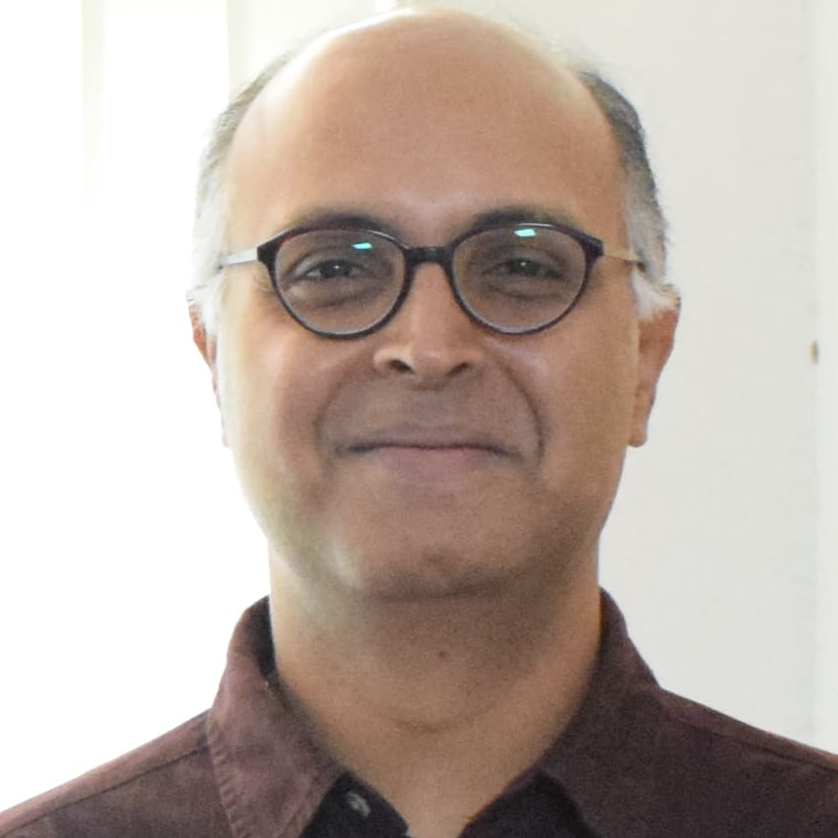
\includegraphics[width=0.6\textwidth]{slal.jpg}\\
	\footnotesize{{\bf Siddhartha Lal}\\
	IISER K}
\end{minipage}
\begin{minipage}{0.25\textwidth}
	\centering
	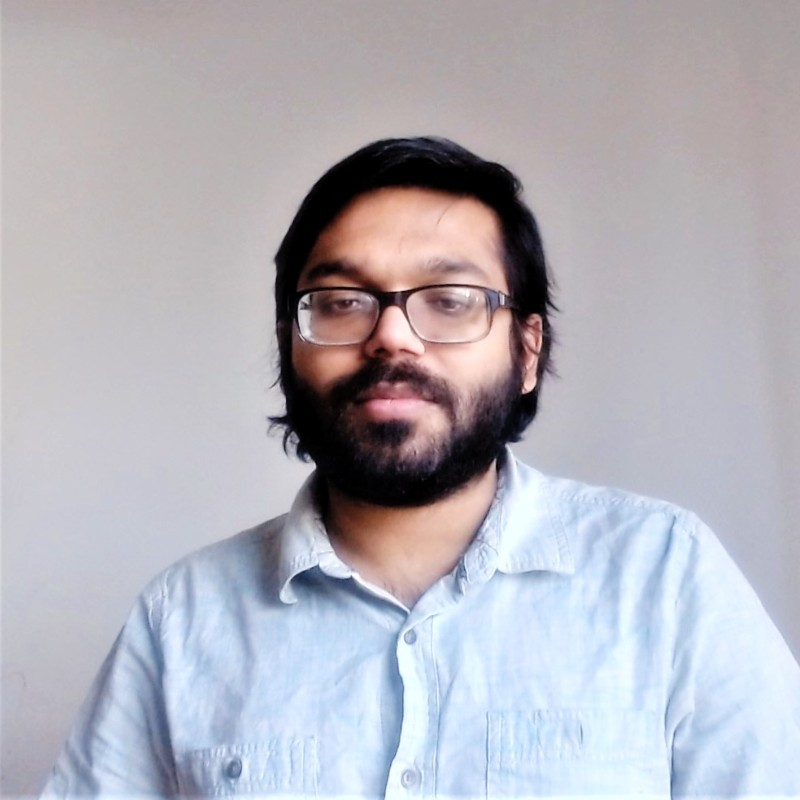
\includegraphics[width=0.6\textwidth]{amukherjee.jpg}\\
	\footnotesize{{\bf Anirban Mukherjee}\\
	IISER K (Graduated)}
\end{minipage}
\begin{minipage}{0.25\textwidth}
	\centering
	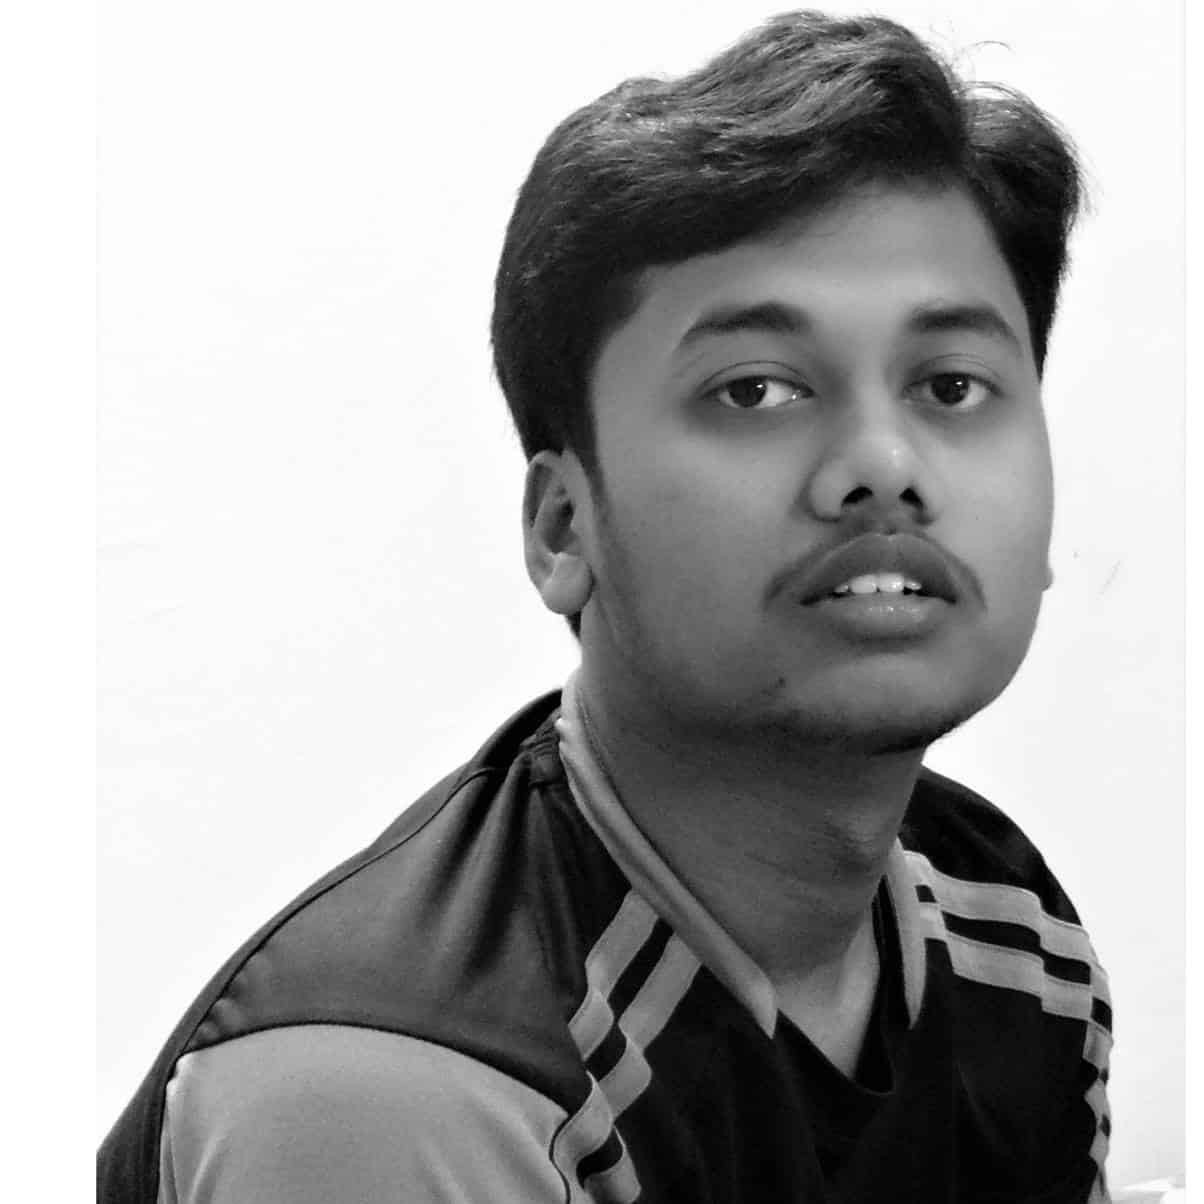
\includegraphics[width=0.6\textwidth]{spatra.jpg}\\
	\footnotesize{{\bf Siddhartha Patra}\\
	IISER K (Graduated)}
\end{minipage}
\begin{minipage}{0.1\textwidth}
	
\includegraphics[width=\textwidth]{dps_logo.jpeg}
\end{minipage}
\hspace*{\fill}
\\
\vspace*{\fill}
\alert{\bf $\sim\sim\sim\sim\sim\sim\sim\sim\sim\sim\sim\sim\sim\sim\sim$ }\\
\alert{\bf A huge thanks to all my collaborators! }\\
\alert{\bf $\sim\sim\sim\sim\sim\sim\sim\sim\sim\sim\sim\sim\sim\sim\sim$ }\\
\vspace*{\fill}

\hspace*{\fill}
\begin{minipage}{0.1\textwidth}
	
\includegraphics[width=\textwidth]{IITKGP.png}\\
\end{minipage}
\hspace*{\fill}
\begin{minipage}{0.3\textwidth}
	\centering
	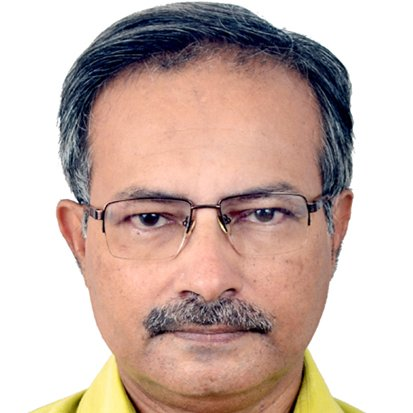
\includegraphics[width=0.45\textwidth]{arghya.jpg}\\
	\footnotesize{{\bf Arghya Taraphder}\\
	IIT Kharagpur}
\end{minipage}
\hspace*{\fill}
\begin{minipage}{0.3\textwidth}
	\centering
	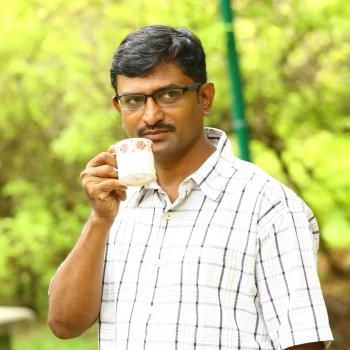
\includegraphics[width=0.45\textwidth]{nsv.jpeg}\\
	\footnotesize{{\bf N. S. Vidhyadhiraja}\\
	JNCASR Bangalore}
\end{minipage}
\hspace*{\fill}
\begin{minipage}{0.1\textwidth}
	
\includegraphics[width=\textwidth]{JNCASR.png}\\
\end{minipage}
\hspace*{\fill}

\end{frame}

\section{Introducing the Kondo effect}
\subsection{Where it all began}

\begin{frame}{What is the Kondo effect?}
\begin{itemize}
	\item metal resistivity is expected to decrease monotonically with temperature: \(\rho \sim T^n\)
	\item metals with magnetic impurities show an anomalous resistivity minimum
\end{itemize}

\footcite{deHaas1939}
	\begin{figure}[htpb]
		\centering
		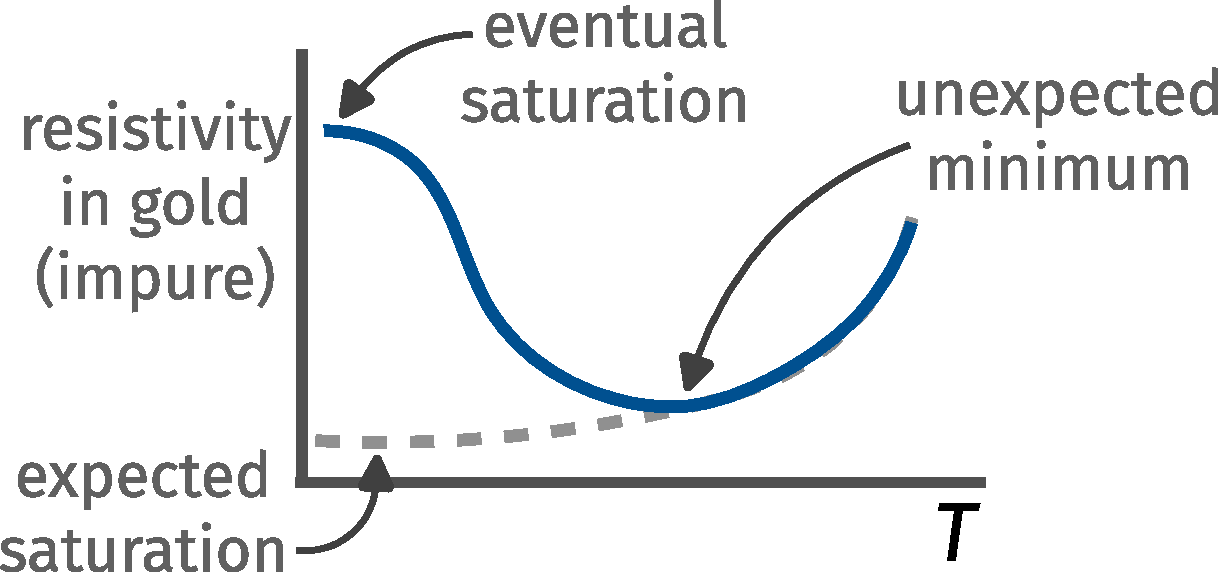
\includegraphics[width=0.45\textwidth]{resistance_minimum.pdf}
		\hspace*{\fill}
		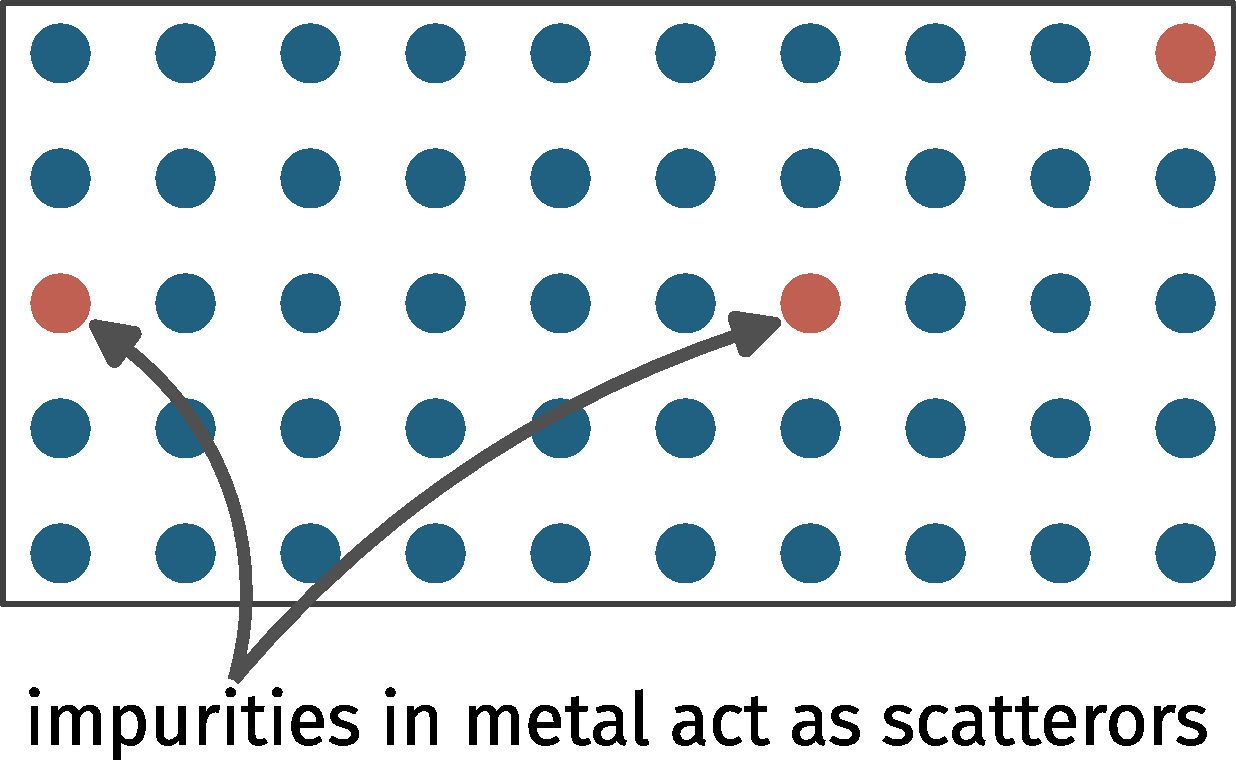
\includegraphics[width=0.45\textwidth]{metal_impurity.pdf}
	\end{figure}
\end{frame}

\begin{frame}{How to explain the resistivity minimum?}
	\begin{figure}[htpb]
		\centering
		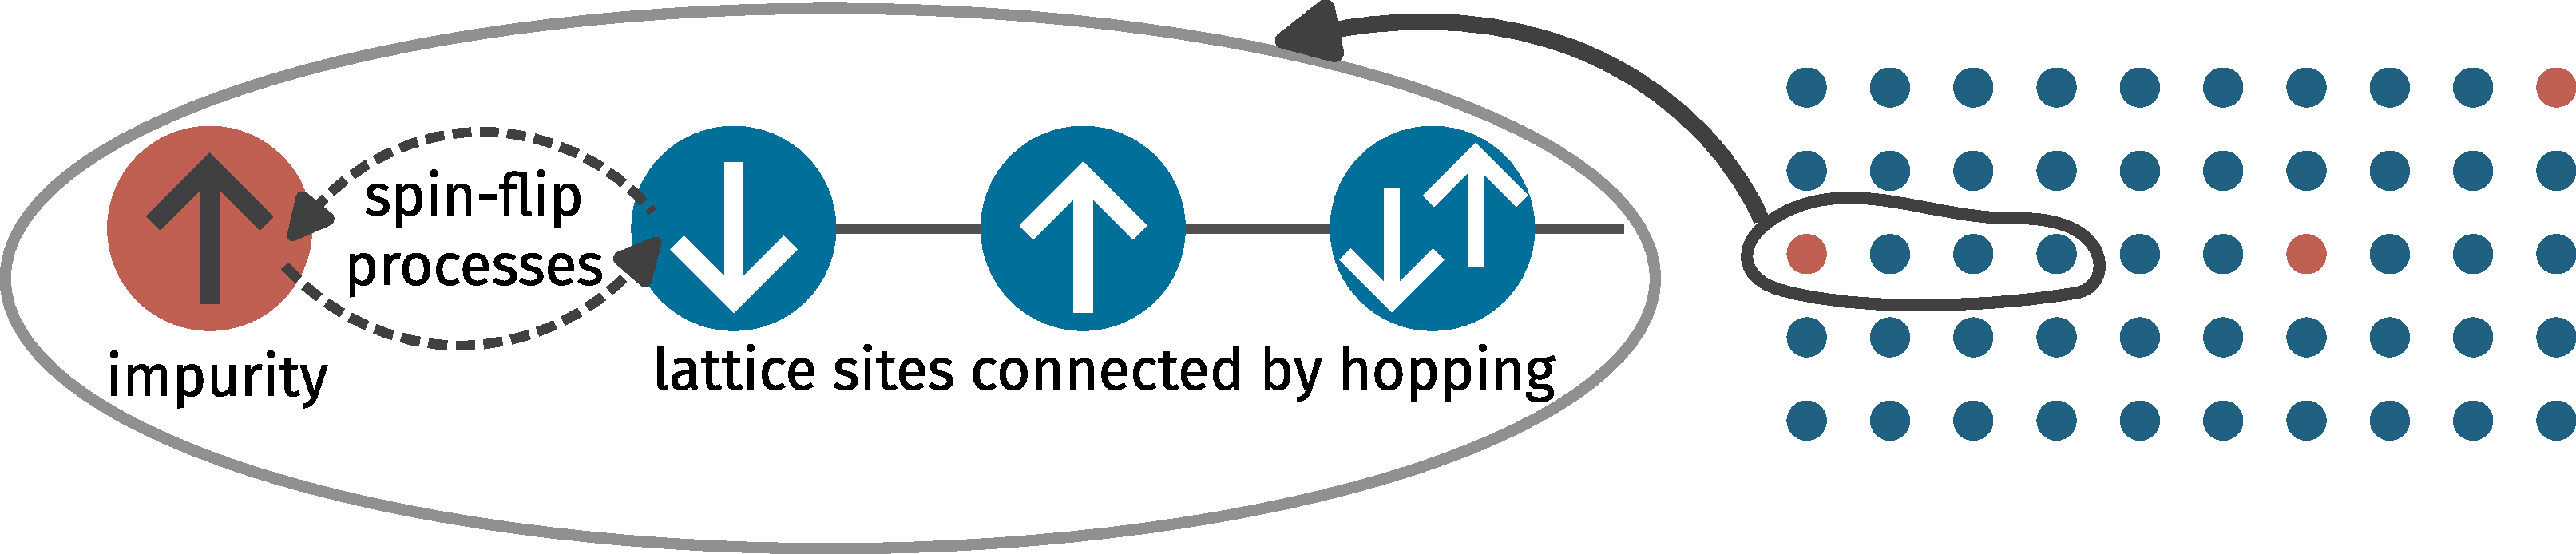
\includegraphics[width=\textwidth]{KondoModel.pdf}
	\end{figure}
\end{frame}

\section{The single-channel Kondo problem}
\subsection{Anatomy of the Kondo cloud}

\section{Distorting the Kondo singlet}
\subsection{The multi-channel Kondo Problem}

\section{How to destroy the Kondo cloud}
\subsection{Effect of local interactions in the bath}

\end{document}
